
\documentclass[12pt]{article}


\input{macros}

\usepackage{pgf}
\usepackage{tikz}

\begin{document}

\def\blattno{6}
\setcounter{uebno}{0}
\renewcommand{\datum}{}
\renewcommand{\beschreibung}{Seminar \blattno}




\newpage

\pagestyle{empty}
\setcounter{page}{1}
\pagestyle{plain}

%\renewcommand{\solution}[1]{}





\renewcommand\thefigure{\arabic{figure}}    

\setcounter{figure}{0} 

\titel

\semex
Give an example where feasible circulations do not exist.
\solution{We consider the following example

\begin{figure}[h!]

\begin{center}
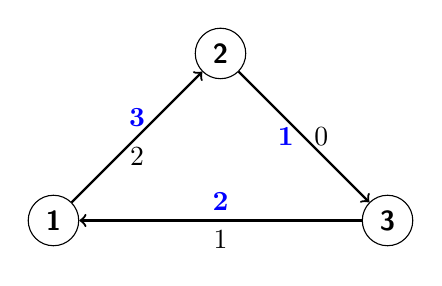
\begin{tikzpicture}
  [normal node/.style={node distance=3cm, circle,fill=white!20,draw,font=\sffamily\bfseries}]
  
\node[normal node] (1){1};
\node[normal node] (2)[above right of=1] {2};
\node[normal node] (3) [below right of=2] {3};
   
\path
  (1) edge [->, thick] node [above] {\textcolor{blue}{$\mathbf{3}$}} node [below] {2} (2)
  (3) edge [->, thick] node [above] {\textcolor{blue}{$\mathbf{2}$}} node [below] {1} (1)
  (2) edge [->, thick] node [left] {\textcolor{blue}{$\mathbf{1}$}} node [right] {0} (3);

\end{tikzpicture}
\end{center}
\end{figure}
Thus, 
\be
\item $D=(V,A)$, where $V=\{1,2,3\}, A=\{(1,2), (2,3), (3,1)\}$,
\item $c((1,2))=3, c((2,3))=1, c((3,1))=2$ and 
\item $d((1,2))=2, d((2,3))=0, d((3,1))=1$. 
\ee
Let $f:A\to\R$ be feasible w.r.t. $d,c$. Then 
$in_f(2)=f((1,2))\geq d((1,2))=2$, while $out_f(2)=f((2,3))\leq c((2,3))=1$. Thus, $in_f(2)\ne out_f(2)$,
so $f$ cannot be a circulation.
}

\semex 
Let $N=(D,s,t)$ be a unit capacity network, $k\geq 1$ and $P_1,\ldots, P_k$ be $k$ 
arc-disjoint $s$-$t$ paths in $D$. Then for all $k\geq 1$, 
\[f:=\chi^{P_1}+\ldots+\chi^{P_k}\]
is an $s$-$t$ $\{0,1\}$-flow $f$ with $\text{value}(f)=k$.
\solution{
For $k=1$, we have that $f:=\chi^{P_1}$ is an $s$-$t$  $\{0,1\}$-flow  of value 1, by (S5.4). 

Let $k\geq 2$. By (S5.4) and Lemma 3.3.2, we have that $f$  satisfies the flow conservation law at every $v\ne s,t$ and $\text{value}(f)=k$. 
It remains to prove that
$f$ takes values in $\{0,1\}$. 
For any $a\in A$, we have one of the two cases:
\be
\item $a\notin P_1\cup\ldots\cup P_k$, so $f(a)=0$.
\item there exists a unique $i=1,\ldots, k$ such that $a\in P_i$, so $f(a)=1$.
\ee
Thus, $f:A\to\{0,1\}$ is a flow. 
}


\semex
Let $D=(V,A)$ be a digraph.  Prove that 
\be 
\item\label{prop-s-t-cut-disconnect-1} Each $s$-$t$ cut is an $s$-$t$ disconnecting arc set.
\item\label{prop-s-t-cut-disconnect-2} Each $s$-$t$ disconnecting arc set of minimum size is an $s$-$t$ cut.
\item The minimum size of an $s$-$t$ disconnecting arc set coincides with the minimum size of an $s$-$t$ cut.
\ee
\solution{
\be
\item Let $\delta^{out}(U)$ be an $s$-$t$ cut, where $s\in U$ and $t\notin U$. Let $P=sv_1\ldots v_kt$ be
an $s$-$t$ path and denote $v_0:=s$ and $v_{k+1}:=t$.  We have two cases:
\be
\item there exists $i=1,\ldots, k$ such that $v_i\notin U$ and $v_{i-1}\in U$. Then $(v_{i-1},v_i)\in \delta^{out}(U)$.
\item $v_i\in U$ for all $i=1,\ldots, k$. Then $(v_k,t)\in \delta^{out}(U)$.
\ee
\item Let $B$ be an $s$-$t$ disconnecting arc set of minimum size. Define  $U$ as the the set of vertices in $V$ accessible from $s$ by paths that contain no 
arcs of $B$. Then $s\in U$ and $t\notin U$, since $B$ is $s$-$t$ disconnecting. 
Hence, $\delta^{out}(U)$ is an $s$-$t$ cut, hence it is an $s$-$t$ disconnecting arc set, by \eqref{prop-s-t-cut-disconnect-1}.

{\bf Claim:} $\delta^{out}(U)\se B$

\solclaim{ Let $a=(u,v)\in \delta^{out}(U)$. Since $u\in U$, there exists an $s$-$u$ path $P$ containing no arcs of $B$.
If $a\notin B$, then $P+a$ is an $s$-$v$ path  containing no arcs of $B$, hence $v\in U$, which is a contradiction with the fact that $(u,v)\in \delta^{out}(U)$.
Thus, $a\in B$. }

By the fact that $B$ is of minimum size, we must have $B=\delta^{out}(U)$.
\item Let $m$ be the first minimum and $m'$ be the second minimum. We have that $m\leq m'$ 
by \eqref{prop-s-t-cut-disconnect-1} and that $m\geq m'$ by \eqref{prop-s-t-cut-disconnect-2}.
\ee
}



\semex
Prove that the incidence matrix $M$  of a directed graph $D = (V,A)$ is totally unimodular.
\solution{
Let $B$ be a square submatrix of $M$ of order $t$. We prove  by induction on $t$ that 
$\det(B)$ is $-1$, $0$ or $1$. The case $t=1$ is trivial. Let $t>1$. We have the following cases:
\be
\item $B$ has a column with only zeros.  Then obviously  $\det(B) = 0$. 
\item $B$ has a column with exactly one nonzero, which is $\pm 1$.   Expand the determinant by this column and use 
the induction hypothesis to conclude that $\det(B)\in \{-1, 0, 1\}$.
\item Each column of $B$ contains two nonzeros, one of them $1$ and the other $-1$. Then 
the sum of all lines of $B$ is $\ov$, hence the lines of $B$ are linearly dependent. As a 
consequence, $\det(B) = 0$.
\ee
}

\end{document}




\end{document}